\documentclass{beamer}
\usepackage{transparent}
\usepackage[beamer]{shortcut}


\usepackage[autoplay]{animate}
\usepackage{bibentry}
\usepackage{subcaption}
\usepackage{stackengine}
\usepackage{appendixnumberbeamer}

\graphicspath{{./images/}}
\def\TikzLocation{./tikz/}
\def\tkzscl{1}

\def\stackalignment{l}


\definecolor{primary}{RGB}{191,213,219}
\definecolor{secondary}{RGB}{144,106,66}
\setbeamercolor{block title}{fg=darkred}
\newcommand{\btitle}[1]{{\usebeamerfont{block title}\usebeamercolor[fg]{block title} #1}}

\AtBeginSection[]
{
}


\makeatletter
\def\beamer@newblock{%
  \usebeamercolor[fg]{bibliography entry author}%
  \usebeamerfont{bibliography entry author}%
  \usebeamertemplate{bibliography entry author}%
  \def\newblock{%
    \usebeamercolor[fg]{bibliography entry title}%
    \usebeamerfont{bibliography entry title}%
    \usebeamertemplate{bibliography entry title}%
    \def\newblock{%
      \usebeamercolor[fg]{bibliography entry location}%
      \usebeamerfont{bibliography entry location}%
      \usebeamertemplate{bibliography entry location}%
      \def\newblock{%
        \usebeamercolor[fg]{bibliography entry note}%
        \usebeamerfont{bibliography entry note}%
        \usebeamertemplate{bibliography entry note}}}}%
  \leavevmode\setbox\beamer@tempbox=\hbox{}\ht\beamer@tempbox=0em\box\beamer@tempbox}
  \setbeamertemplate{bibliography entry title}{}{}

\makeatother

\usepackage[square, authoryear]{natbib}


%-----------------------------------------------------------------------------
%	CUSTOM COMANDS
%-----------------------------------------------------------------------------

\def\keypoint#1{\hspace{0pt plus 1 filll}\textcolor{gray}{[{\color{linkcolor}#1}]}~}
\def\mycite#1{\keypoint{\small\citealt{#1}}}
\def\citeconf#1#2{
    {\textcolor{gray}[}%
        {\color{linkcolor}\citealt{#1}, #2}%
    {\textcolor{gray}]}}
\def\citeconfright#1#2{\hspace{0pt plus 1 filll}{\small\citeconf{#1}{#2}~}}
\def\biblio{
	\nobibliography{../../library}
	\def\biblio{}
}

\def\myitem{\hskip1ex{\color{linkcolor} $\blacktriangleright$}\hskip.3em}


\def\extraLogo{\includegraphics[width=.2\linewidth]{brain_and_signals}}


\newlength\bodywd
\newlength\skipg
\setlength\skipg{\widthof{\bf g}}
\newcommand{\techterm}[1]{
    \column{\widthof{\bf #1}}
    \centering
    \begin{beamercolorbox}[rounded=true, shadow=true]{title}
        \bf \phantom{g}\hskip-\skipg #1
    \end{beamercolorbox}
}

\pgfkeys{
    /highlight/.cd,
    c/.initial={darkred},
    wd/.initial={0}
}

\newcommand{\highlight}[2][]{%
    \pgfkeys{/highlight/.cd,#1}%
    \ifthenelse{\pgfkeysvalueof{/highlight/wd}=0}{
        \setlength\bodywd{\widthof{\bf #2}}
    }{
        \setlength\bodywd{\pgfkeysvalueof{/highlight/wd}}
    }
    \raisebox{-.5em}{
        \begin{beamercolorbox}[rounded=true, shadow=true, wd=\bodywd]{title}
            \centering\bf\phantom{g}\hskip-\skipg \textcolor{\pgfkeysvalueof{/highlight/c}}{#2}
    \end{beamercolorbox}}
}

\newcommand{\overimg}[5][.8\linewidth]{
    \begin{tikzpicture}
    \only<#2-#4>{%
        \node[inner sep=0em, outer sep=0em] (img) {\includegraphics[width=#1]{#3}};
    }%
    \only<#4>{%
        \path let
          \p1=($(img.north) - (0, 1em)$), \p2=(img.south)
          in
          node {\includegraphics[height=\y1-\y2]{#5}};
    }%
    \end{tikzpicture}
}


\institute{Concours CRCN Inria Saclay}
\author{Thomas Moreau}
\title{Apprentissage non supervisé pour les signaux multivariés
       en neurosciences}


\setbeamertemplate{title page}[frame]


\begin{document}

\begin{frame}[plain]

\vskip.1\textheight
\begin{beamercolorbox}[sep=2pt,center, wd=\textwidth]{separationline}
    %Title box
    \begin{beamercolorbox}[center, wd=\SizeTitleBox]{headline}
        \begin{center}
            \centering
            \usebeamercolor{title}{\color{fg}\Large\textbf{{\inserttitle}}\hskip2em\\[1.5ex]}
            \usebeamercolor{author}{\color{fg}\small{\insertauthor}} -- %
            \usebeamercolor{institute}{\color{fg}\small{\insertinstitute}\\}
        \end{center}
    \end{beamercolorbox}
    \vskip-1em
    \hskip0em
    % Separation line
    \begin{beamercolorbox}[center, wd=\SizeTitleBox]{separation line}\rule{0pt}{2pt}\end{beamercolorbox}\vfill
\end{beamercolorbox}
% LOGO and join work part of the title frame
\vskip2em
\begin{columns}[c]
    \column{.5\textwidth}
    \centering
        \includegraphics[width=.7\linewidth]{brain_and_signals}
    \column{.5\textwidth}
        \includeLogo{logo_inria}\\[1em]
        \includeLogo{logo_parietal}
\end{columns}


\biblio{}
\end{frame}

\def\biblio{}

%===========================================================================
\section{Me}
%===========================================================================

\begin{frame}[t]{Parcours}

\begin{columns}[c]
    \column{1em}
    \rotatebox{90}{\Large Formation}
    \column{.9\textwidth}
\begin{list}{}{\leftmargin=0em \itemsep=0em}
    \item 2010-2014: Ecole Polytechnique - Maths Appli/Info
    \item 2013-2014: Double diplôme Telecom ParisTech - Master MVA
\end{list}
    \begin{beamercolorbox}[rounded=true, shadow=true]{title}
       Apprentissage statistique, Traitement du signal et des images
    \end{beamercolorbox}
\end{columns}

\vskip1em

\begin{columns}[c]
    \column{1em}
    \rotatebox{90}{\Large Recherche}
    \column{.9\textwidth}
    \begin{list}{}{\leftmargin=0em \itemsep=1em}
        \item 2014-2017: Thèse -- ENS Cachan (N. Vayatis \& L. Oudre)
        \vskip-.5em
        \begin{columns}[T]
            \column{.45\textwidth}
        \begin{block}{\bf Maths appliquées}\footnotesize
            Optimisation distribuée\\
            Apprentissage non supervisé\\
            Apprentissage de représentation
        \end{block}
        \column{.01\textwidth}
        \column{.45\textwidth}
        \begin{block}{\bf Données de Santés}\footnotesize
            Analyse de la marche\\
            Enregistrements oculomoteurs
        \end{block}

        \end{columns}

        \item 2018-2019: Post-doctorat -- Inria (équipe Parietal) \keypoint{15 mois}\\
        \begin{beamercolorbox}[rounded=true, shadow=true]{title}
            {\bf Apprentissage de dictionnaire convolutif pour la MEG}\\[.3em]
            \hskip3ex\color{black}$\Rightarrow$ Analyse de la {\bf structure locale} des signaux
        \end{beamercolorbox}
    \end{list}
\end{columns}

\end{frame}


\begin{frame}{Analyse de l'équilibre dynamique (Travail Doctoral)}

\begin{columns}[T]
    \column{.58\textwidth}
    \centering
        \begin{columns}[c]
            \column{.4\linewidth}
            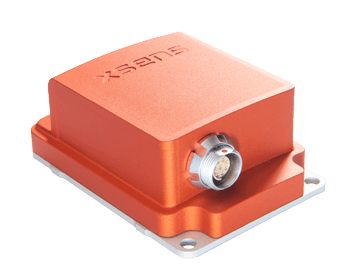
\includegraphics[width=\linewidth]{xsens}
            \column{.6\linewidth}
            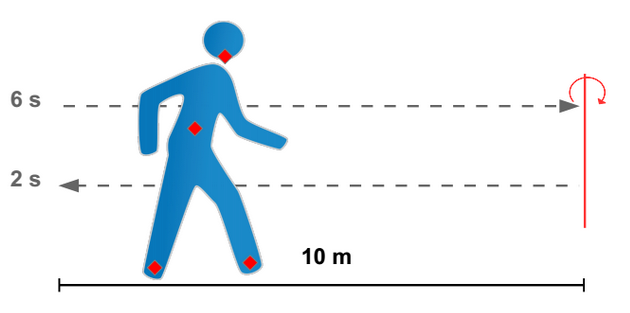
\includegraphics[width=\linewidth]{exo_marche}
        \end{columns}
        {\tiny Enregistrement d'un sujet témoin (Hôpital Militaire de Percy)}
        \only<1>{%
            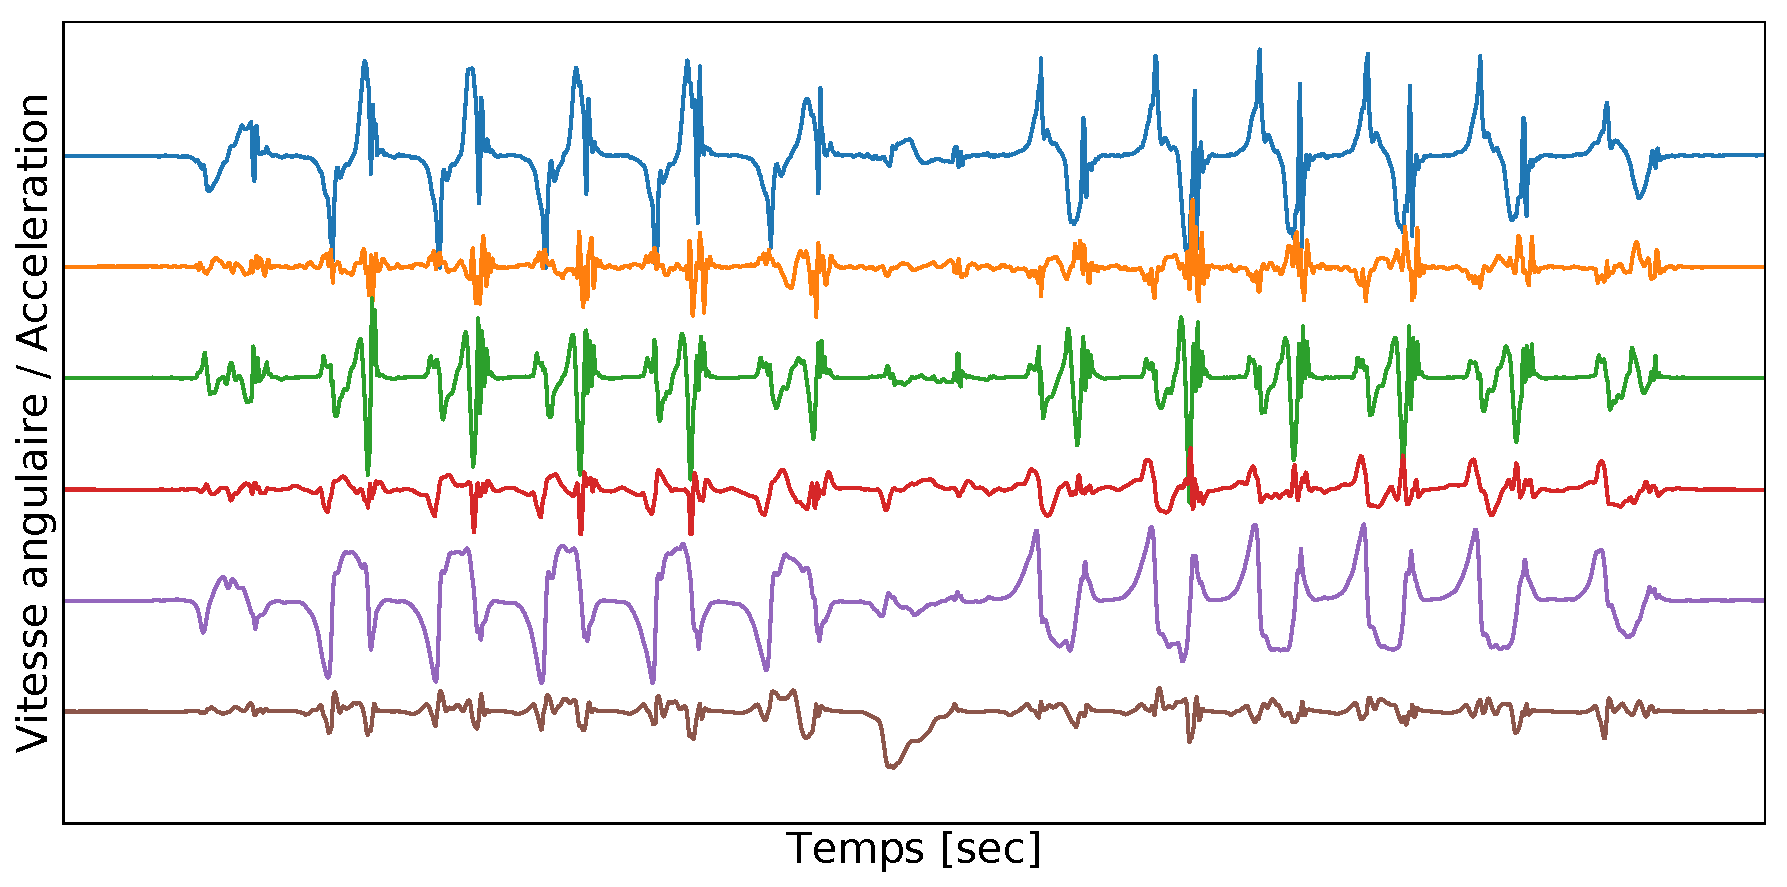
\includegraphics[width=\linewidth]{accelero}
        }
        \only<2-3>{%
            \overimg[\linewidth]{2}{accelero_steps}{3}{accelero_dict}
        }
        \vskip-1em\hskip.5ex
        \begin{beamercolorbox}[rounded=true, shadow=true, wd=.95\linewidth]{title}
            \textbf{Brevet:~} \textcolor{black}{Segmentation de pas}\\
            \textbf{Articles:} %
                \textcolor{linkcolor}{Sensors 2018; PLoS One 2016}\\
        \end{beamercolorbox}
    \column{.4\textwidth}
            \begin{block}{\bf Quantifier de l'équilibre}
                \vskip.5em
                \begin{itemize}\itemsep.5em
                    \item Prédiction de chutes
                    \item Suivi des neuropathies
                \end{itemize}
               \vskip-.7em\textcolor{white}{.}
            \end{block}
            \begin{block}{\bf Challenges}
                \vskip.3em
                Annotations faibles\\[.5em]
                Comparaison des signaux
                \vskip-.7em\textcolor{white}{.}
            \end{block}
            \begin{block}{\bf Comparaison des signaux}
                \vskip.5em
                Représentation adaptée\\[.5em]
                {\bf Structure locale} $\Rightarrow$ le pas
                \vskip-.7em\textcolor{white}{.}
            \end{block}
    \end{columns}

\end{frame}


\begin{frame}{Autres domaines d'application (Post-Doc)}{}
    {\large \bf Image du Télescope Hubble}\\[1em]
    \centering
    \overimg{1}{Hubble}{2}{Hubble_dict}\\[1em]
    \textcolor{gray}{[\textcolor{linkcolor}{preprint 2019}]}
\end{frame}



\begin{frame}{Autres domaines d'application (Post-Doc)}{}
    {\large \bf Magnétoencéphalographie (MEG)}\\[1em]
    \begin{columns}[T]
        \column{.4\textwidth}
            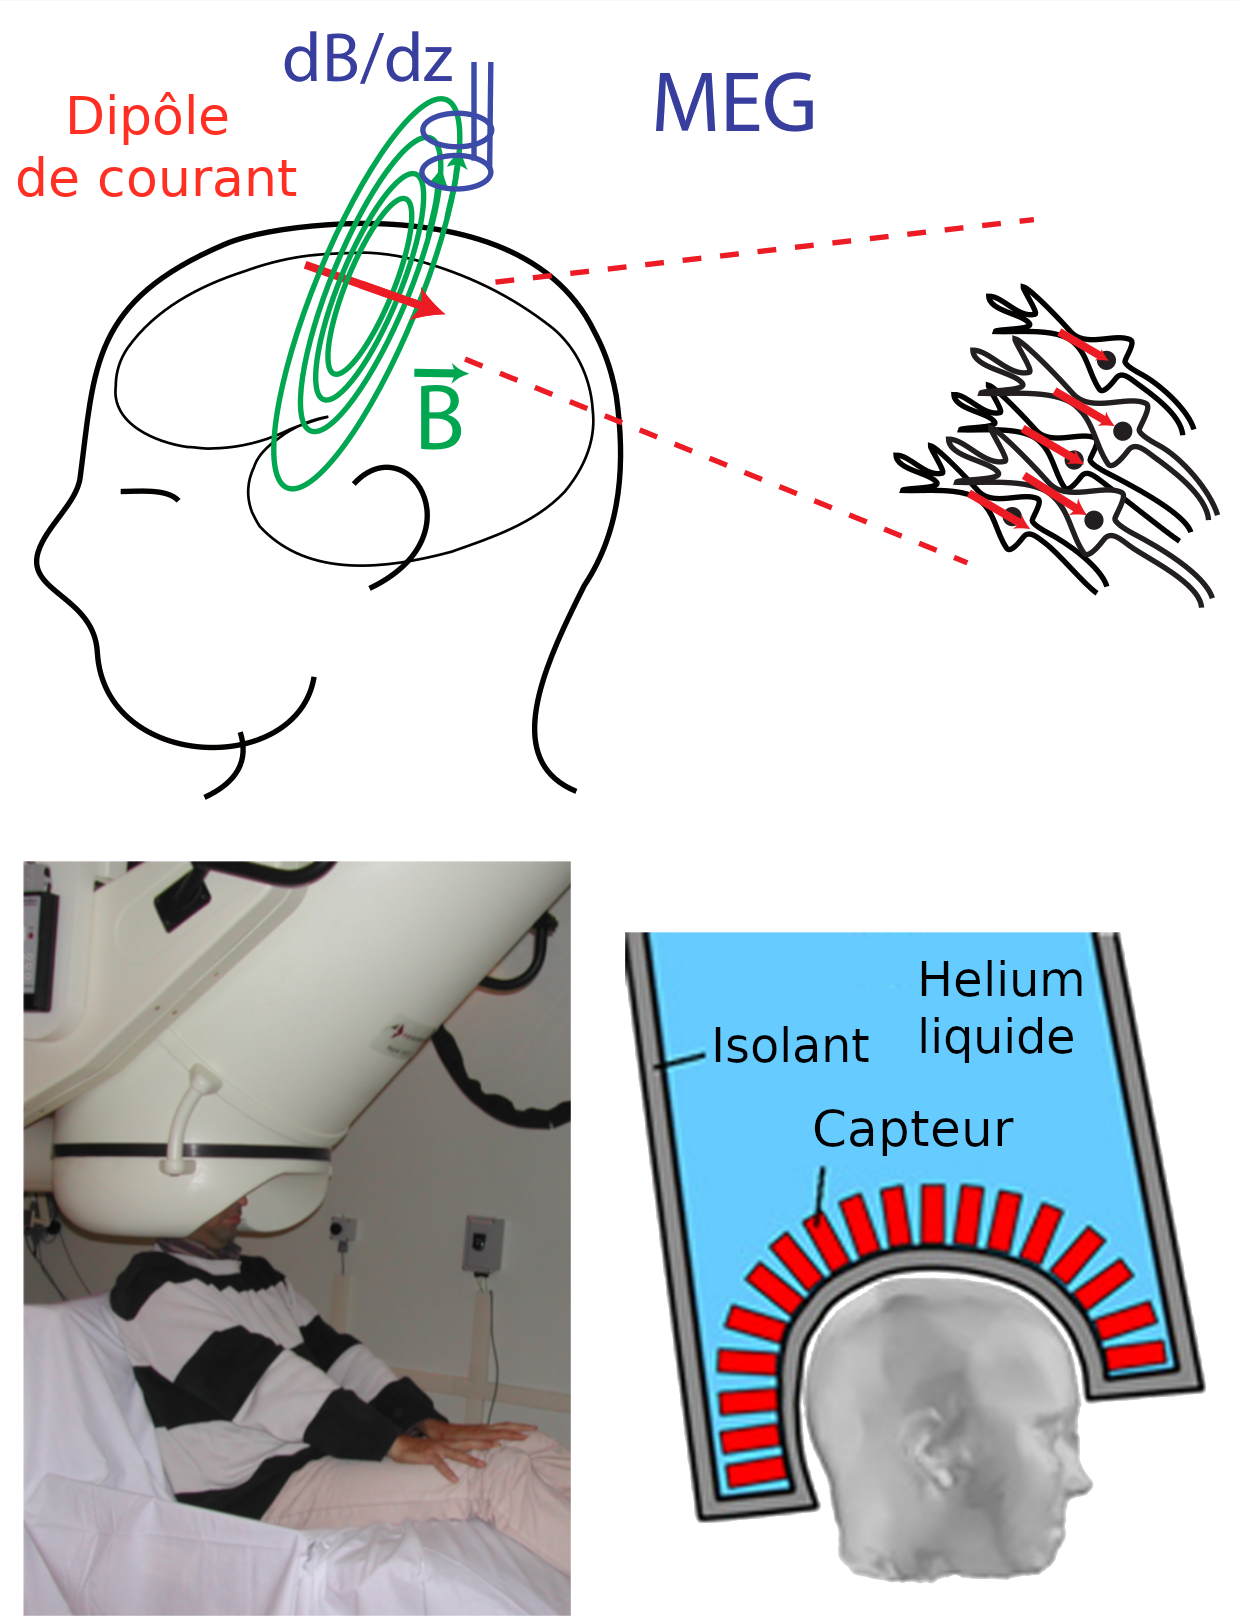
\includegraphics[height=.7\textheight]{meg_presentation}\\
        \column{.6\textwidth}
            {\vskip-3em\centering\hskip4em 
\includegraphics[height=1.5em]{logo_parietal}\\}\vskip3em
            \centering\highlight[c=linkcolor]{Structure locale non distinguable}\\
            \overimg[\linewidth]{1}{meg_signal}{2}{meg_dict}
            \uncover<2>{\textcolor{gray}{[\textcolor{linkcolor}{NeurIPS 2018, ICASSP 2019}]}}
    \end{columns}
\end{frame}

\begin{frame}[t]{Structure locale des signaux}
    \vskip1.5em%
    \centering%
    \only<1>{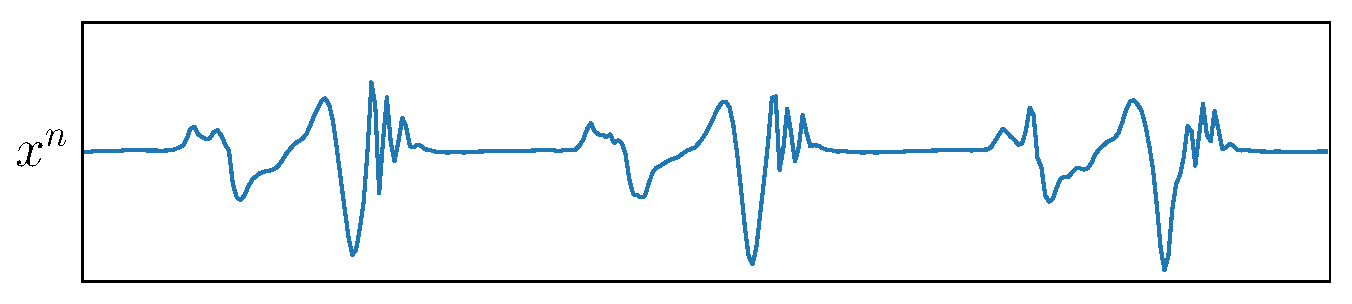
\includegraphics[width=\textwidth]{intro_csc_0}}%
    \only<2>{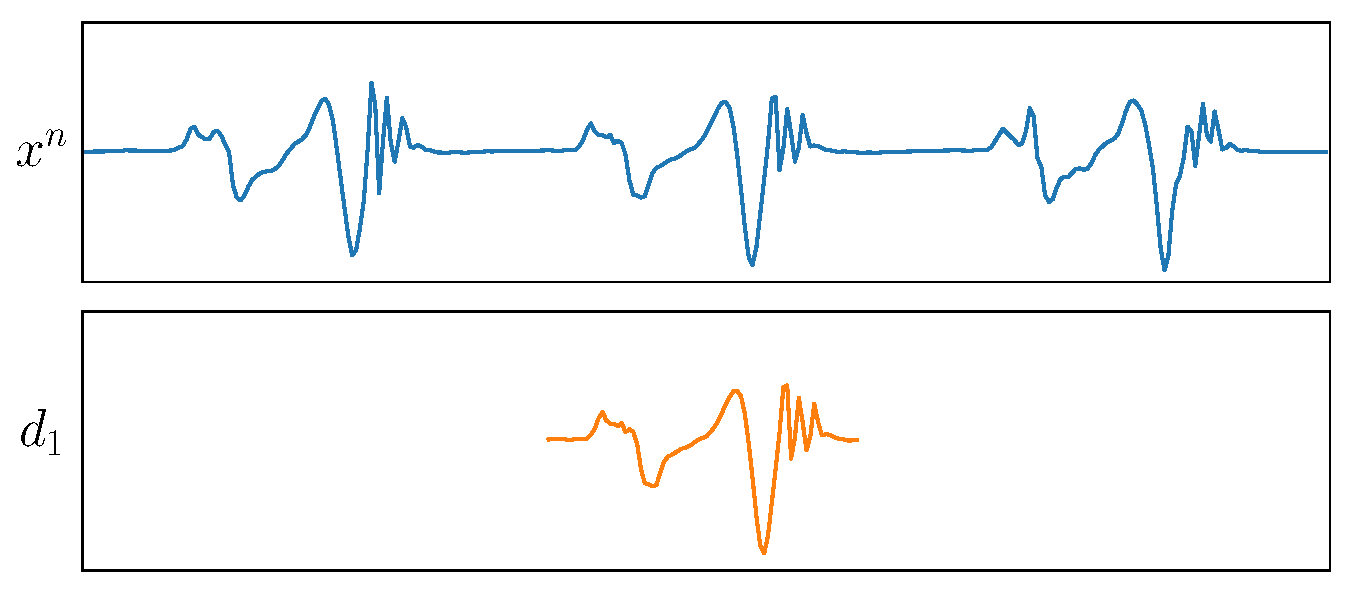
\includegraphics[width=\textwidth]{intro_csc_1}}%
    \only<3>{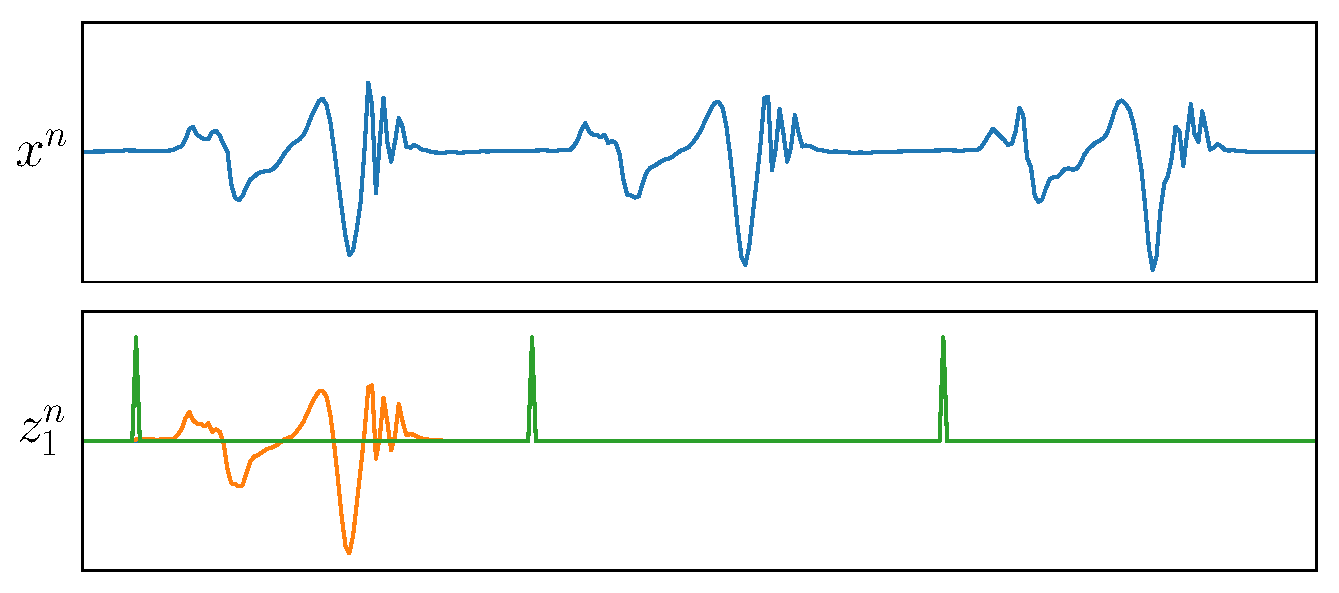
\includegraphics[width=\textwidth]{intro_csc_2}}%
    \only<4>{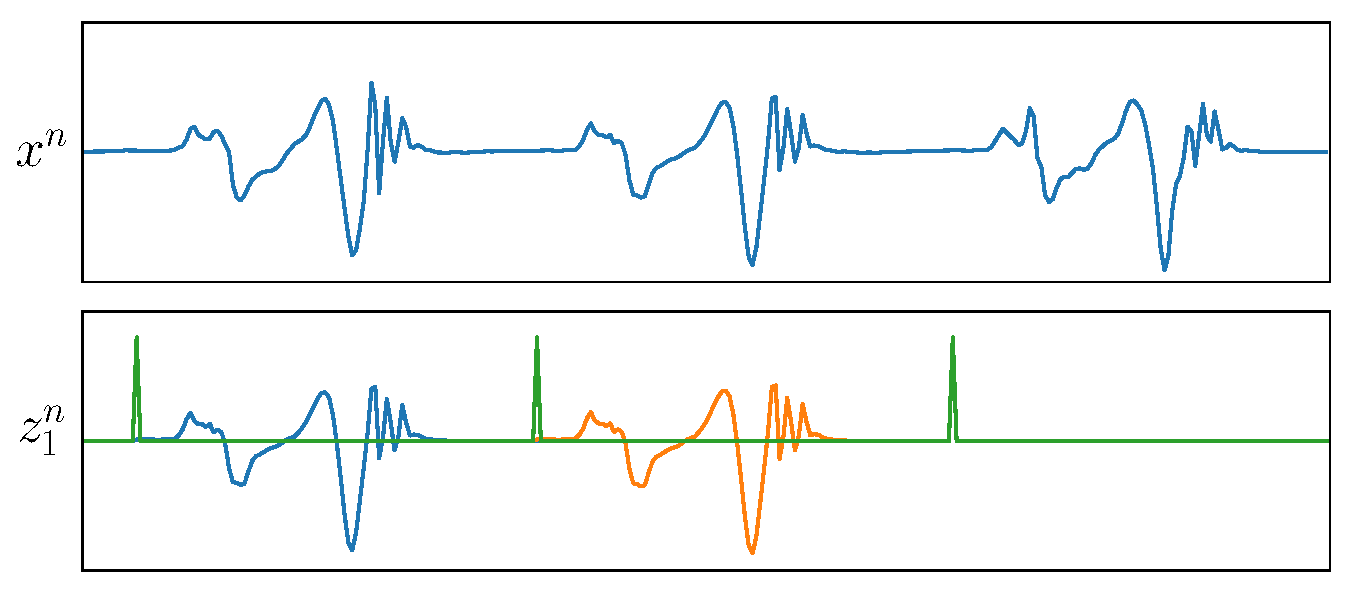
\includegraphics[width=\textwidth]{intro_csc_3}}%
    \only<5>{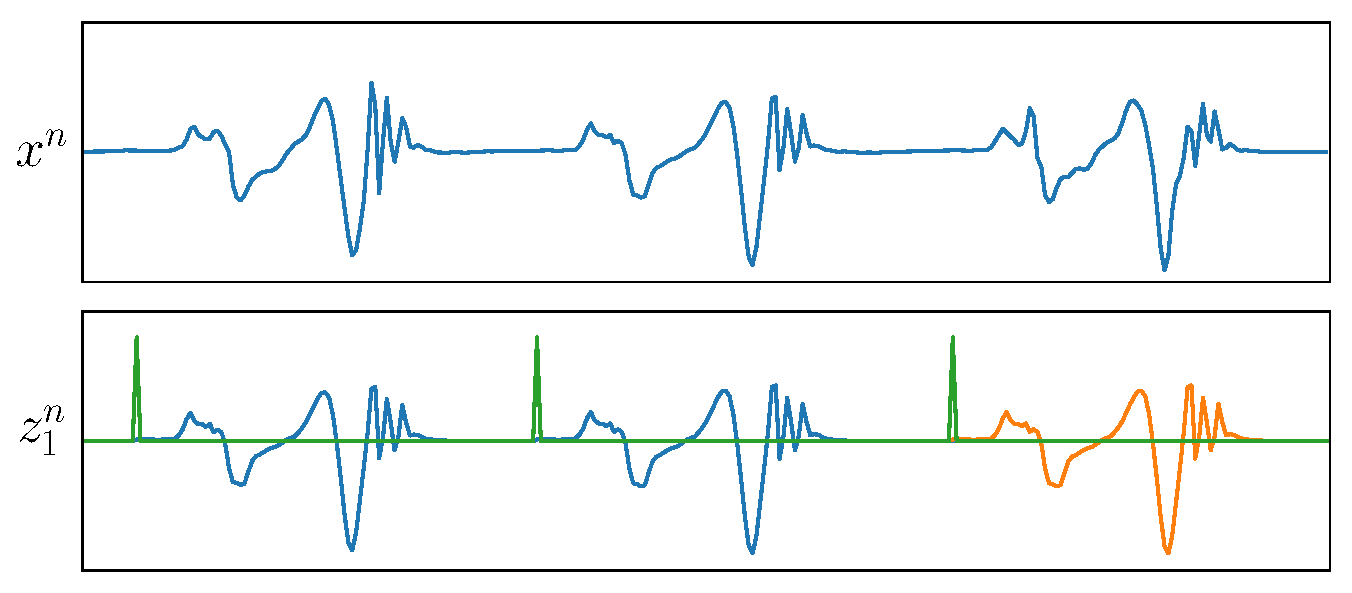
\includegraphics[width=\textwidth]{intro_csc_4}}%
    \only<6->{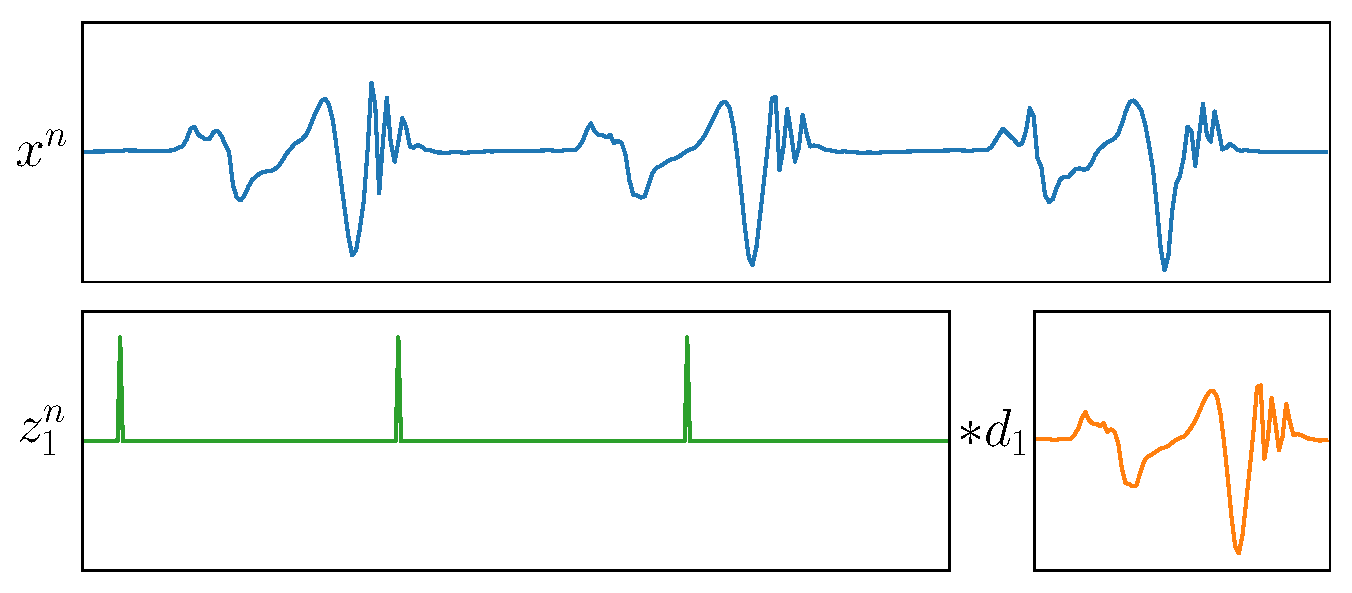
\includegraphics[width=\textwidth]{intro_csc_5}}%
    \vskip.2em%
    \only<7>{%
        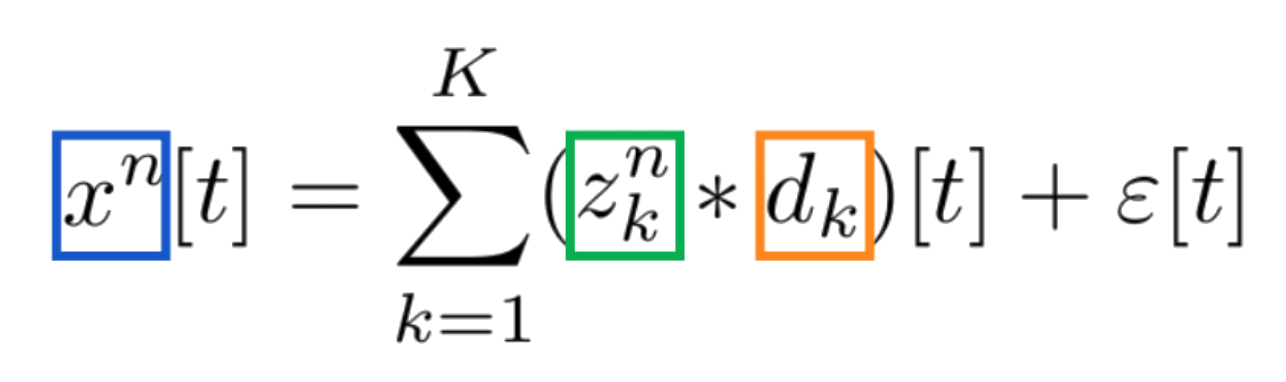
\includegraphics[width=.6\textwidth]{csc_explain_eq_color}%
    }
\end{frame}

\begin{frame}{Challenges de l'apprentissage non supervisé pour les signaux}

    \centering
    \setlength\bodywd{.95\linewidth}
    \highlight[wd=\bodywd, c=black]{\raggedright\textcolor{darkred}{\bf Computationnel:}
        \normalfont passage à l'échelle pour les longs signaux,\\[-.2em]
        \begin{itemize}\color{black}\itemsep0em
            \item[$\bullet$] Parallélisation%
                             \keypoint{ICML 2018; preprint 2019}
            \item[$\bullet$] Utilisation de la structure du dictionnaire%
                             \keypoint{ICLR 2017}
        \end{itemize}%
    }\vskip.5em
    \highlight[wd=\bodywd, c=black]{\raggedright\textcolor{darkred}{\bf Modélisation:}
        \normalfont incorporer de la connaissance du domaine,\\[-.2em]
        \begin{itemize}\color{black}\itemsep0em
            \item[$\bullet$] Activations structurées%
            \keypoint{ICASSP 2019}
            \item[$\bullet$] Motifs structurés%
            \keypoint{NeurIPS 2018}
        \end{itemize}%
    }\vskip.5em
    \highlight[wd=\bodywd, c=black]{\raggedright\textcolor{darkred}{\bf Évaluation:}
        \normalfont analyse statistique des modèles non supervisés,\\[-.2em]
        \begin{itemize}\color{black}\itemsep0em
            \item[$\bullet$] Critères de sélection de modèle%
            \item[$\bullet$] Test de présence des motifs%
        \end{itemize}%
    }\vskip.5em
    \highlight[wd=\bodywd, c=black]{\raggedright\textcolor{darkred}{\bf Théorique:}
        \normalfont garantie de reconstruction des motifs,\\[-.2em]
        \begin{itemize}\color{black}\itemsep0em
            \item[$\bullet$] Lien avec l'apprentissage profond%
            \keypoint{ICLR 2017}
            \item[$\bullet$] Algorithme convergeant globalement%
        \end{itemize}%
    }


\end{frame}

\begin{frame}[t]{Apprentissage de dictionnaire convolutif distribué%
              \keypoint{ICML, 2018}}

{\bf Obstacle computationnel:} Estimation de $Z$ pour un dictionnaire $\pmb D$ fixé\\
    \vskip-.5em
    \[
    \argmin_{Z_k} \| X - \sum_{k=1}^K Z_k * \pmb D_k\|_2^2 + \lambda\sum_{k=1}^K\|Z_k\|_1
    \]
\only<1>{%
    \vskip1em
    {\large \bf Algorithmes existants:}\\[.5em]
    \begin{itemize}\itemsep1em
        \item Descente par Coordonnée Gloutonne\mycite{Kavukcuoglu2013}\\
            % {\small$\mathcal O(K^2T^2/q)$}
            \hskip-5ex\highlight{Complexité \small\color{black}$\mathcal O(K^2T^2/\epsilon)$}
            \hskip3ex{\small Itération $\mathcal O(KT)$
             $\times$ Convergence $\mathcal O(KT/\epsilon)$}
        \item Méthodes globales \mycite{Chalasani2013,Bristow2013}\\
             % {\small$\mathcal O(K^2TL/q)$}
             \hskip-5ex\highlight{Complexité \small\color{black}$\mathcal O(K^2TL/\epsilon)$}
             \hskip3ex{\small Itération $\mathcal O(K^2TL)$
              $\times$ Convergence $\mathcal O(1/\epsilon)$}
    \end{itemize}

}%
\vskip-1em
{
\centering
\inputTikZ{.7}{DICOD}\\[.5em]
}

\only<3->{
{\vskip-.5em\bf Algorithme distribué exact pour les signaux temporels:}
\begin{columns}[c]
    \column{.5ex}
    \techterm{\small Asynchrone}
    \column{.5ex}
    \techterm{\small Communications Locales}
    \column{.5ex}
    \techterm{\small Super linéaire}
    \column{.5ex}
\end{columns}
\vskip-1em% {\bf Super linéaire:}
   {\centering\highlight{\small Complexité \small\color{black}$\small\mathcal O(K^2T^2/{\color{linkcolor}\pmb {W^2}}\epsilon)$}\\
    \only<3>{\vskip.5em\small  Itération $\small\mathcal O(KT/W)$ $\times$ \small Convergence $\small\mathcal O(KT/W\epsilon)$\\}}%
}%
%
\alt<4>{%
       {\vskip.5em\raggedright
       \textcolor{gray}{[{\color{linkcolor}preprint 2019}]} Extension pour signaux 2D + complexité $\small\mathcal O(K^2TL/W\epsilon)$}\\
        \vspace{0pt plus 1 filll}{%
            \centering 
\includegraphics[height=.8em]{github}~\url{github.com/tommoral/dicodile}:
                Implémentation Python + MPI\\}
}{%
\vspace{0pt plus 1 filll}{\small\centering
    $T$: longueur du signal\hskip5ex
    $K$: nombre d'atomes\hskip5ex
    $L$: longueur des atomes\\
    $W$: nombre de noeuds\hskip5ex
    $\epsilon$: précision de la résolution\\}
}

\end{frame}


%\begin{frame}{Application aux Neurosciences \keypoint{NeurIPS, 2018}}
%
%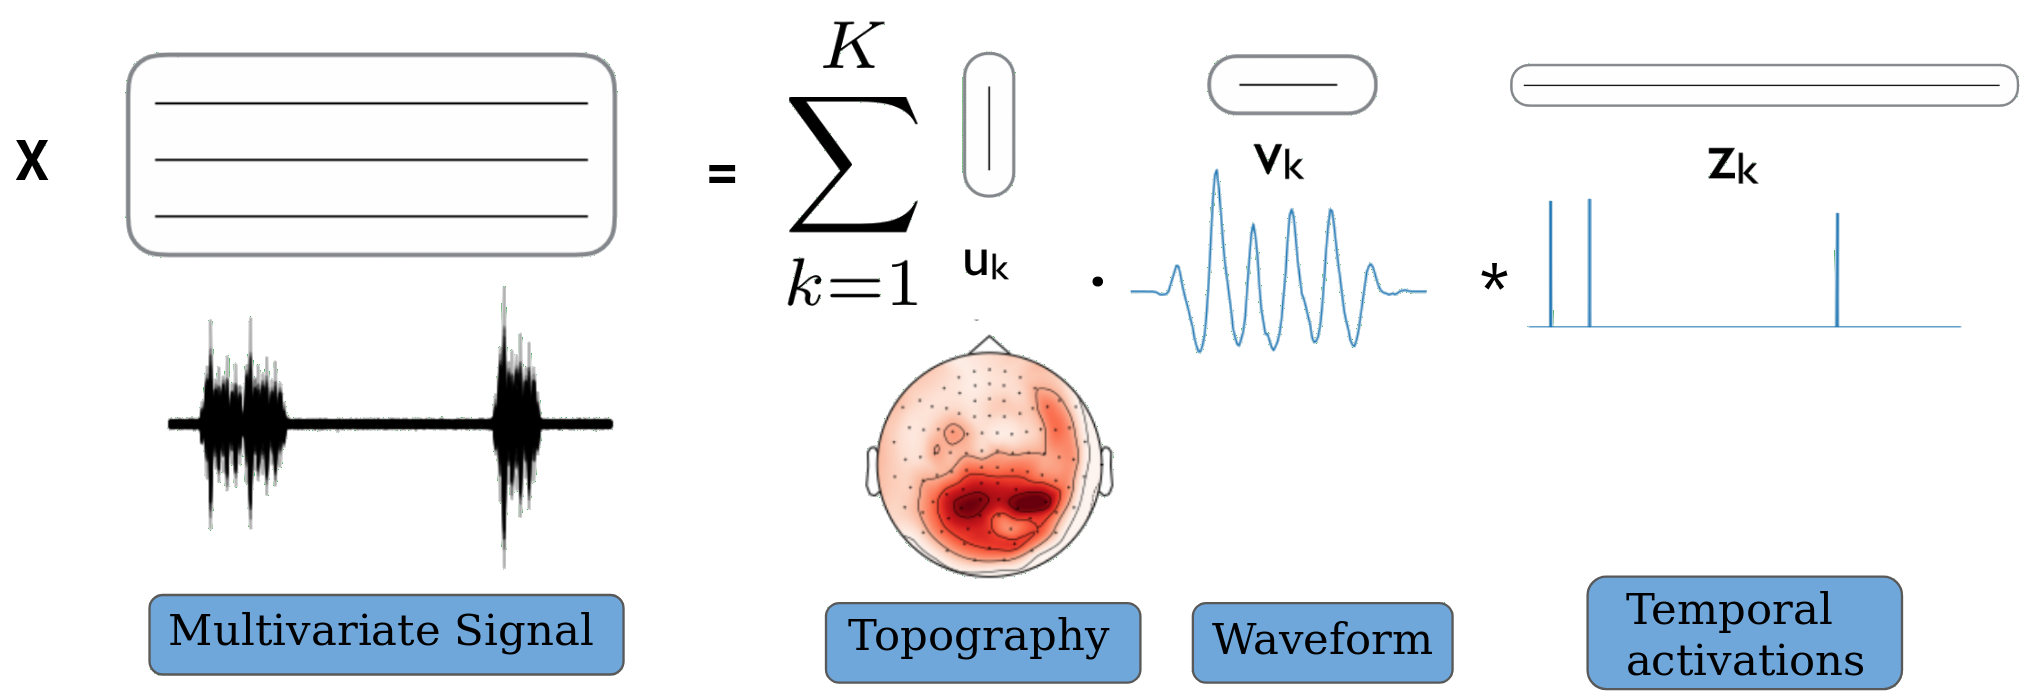
\includegraphics[width=\textwidth]{rank1}
%
%\vskip1em
%\begin{itemize}\itemsep.5em
%    \item Modèle adapté à la physique des signaux MEG,
%    \item Les atomes sont identifiables (réponses évoquées, artefacts, \dots)
%    \item Les activations sont liées à la latence dans les signaux MEG de tâches.
%\end{itemize}
%\vskip3em
%\centering
%
\includegraphics[height=.8em]{github}~\url{alphacsc.github.io}: librairie Python\\[1em]
%\end{frame}


\begin{frame}[t]{Application aux Neurosciences \keypoint{NeurIPS, 2018}}

\centering
\begin{tikzpicture}
    \node (meg) at (0, 0) {
        \alt<1>{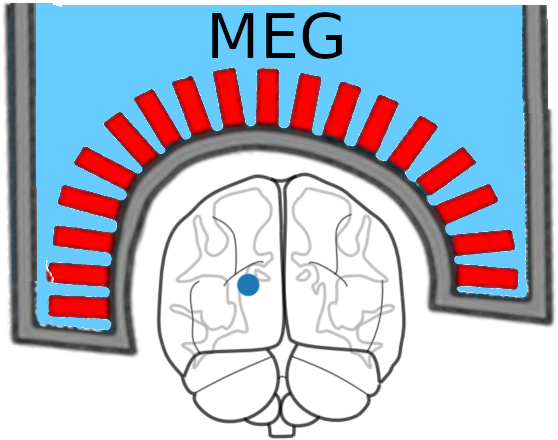
\includegraphics[width=6em]{meg_localised_source}}{%
                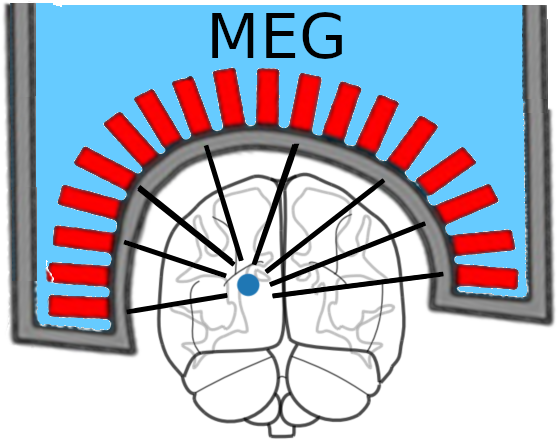
\includegraphics[width=6em]{meg_linear_propagation}}
    };
    \node[right=2em of meg, inner sep=0] (signal) {
        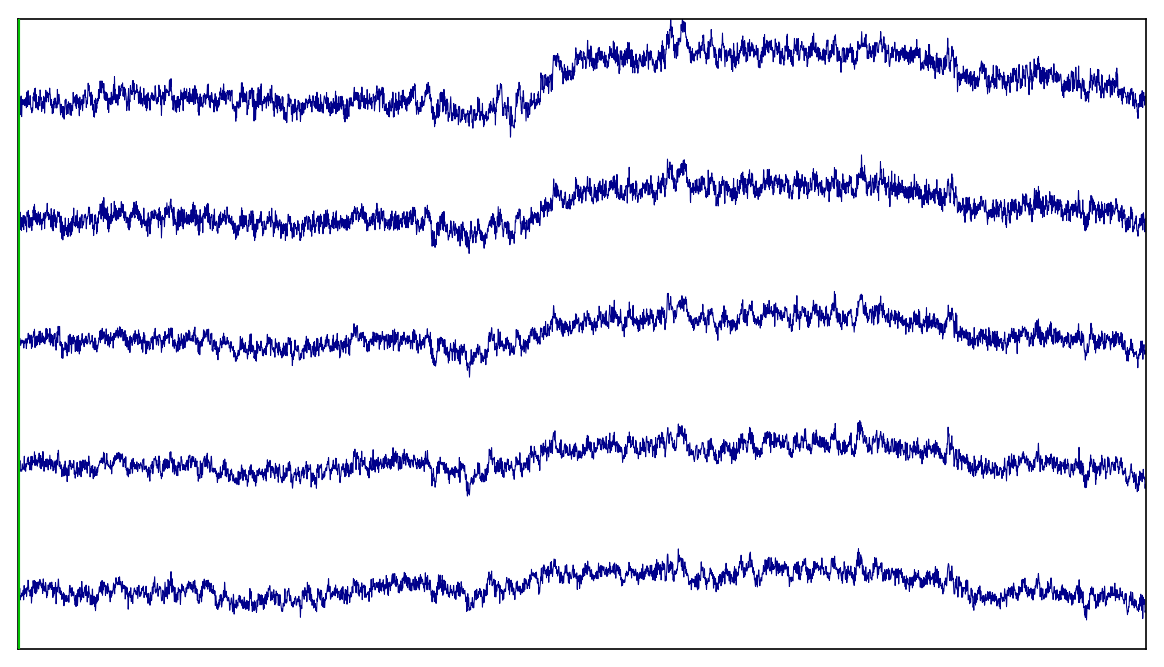
\includegraphics[width=6em]{meg_1}
    };
    \draw[<->, shorten >= 1pt, shorten <= 1pt] (signal.south west) -- (signal.north west)
        node[midway, sloped, above] {\footnotesize Capteurs};
    \uncover<-1>{\node[right=7em of signal] (dict) {%
        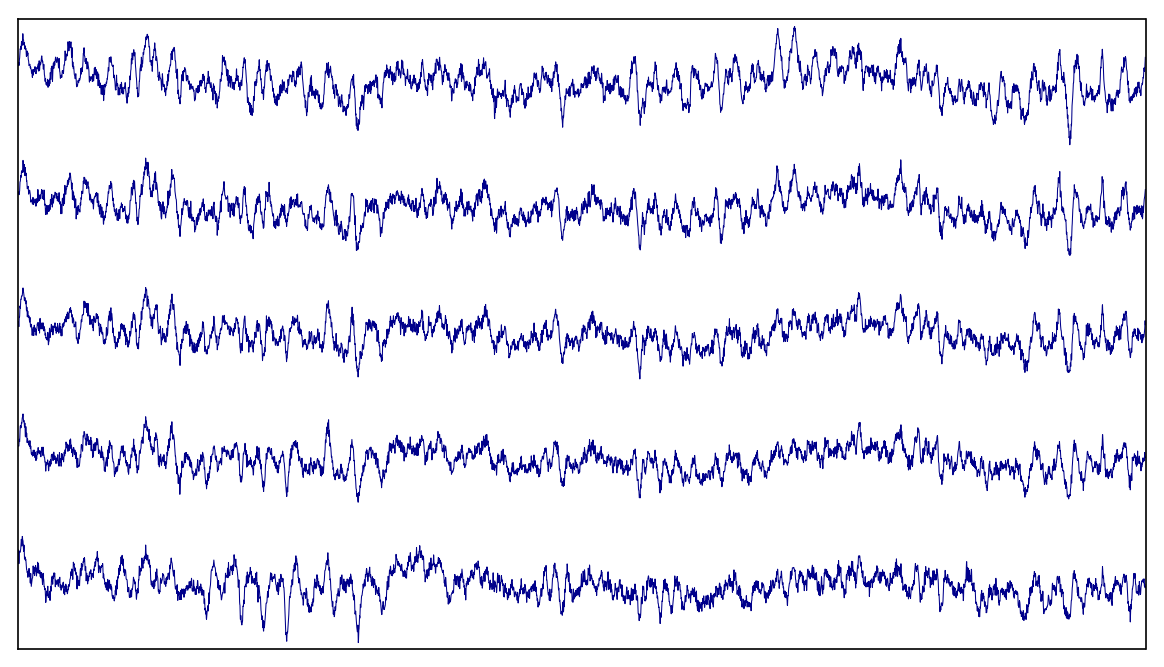
\includegraphics[width=6em]{meg_2}
    };}
    \uncover<2->{\node[right=7em of signal] (dict) {
        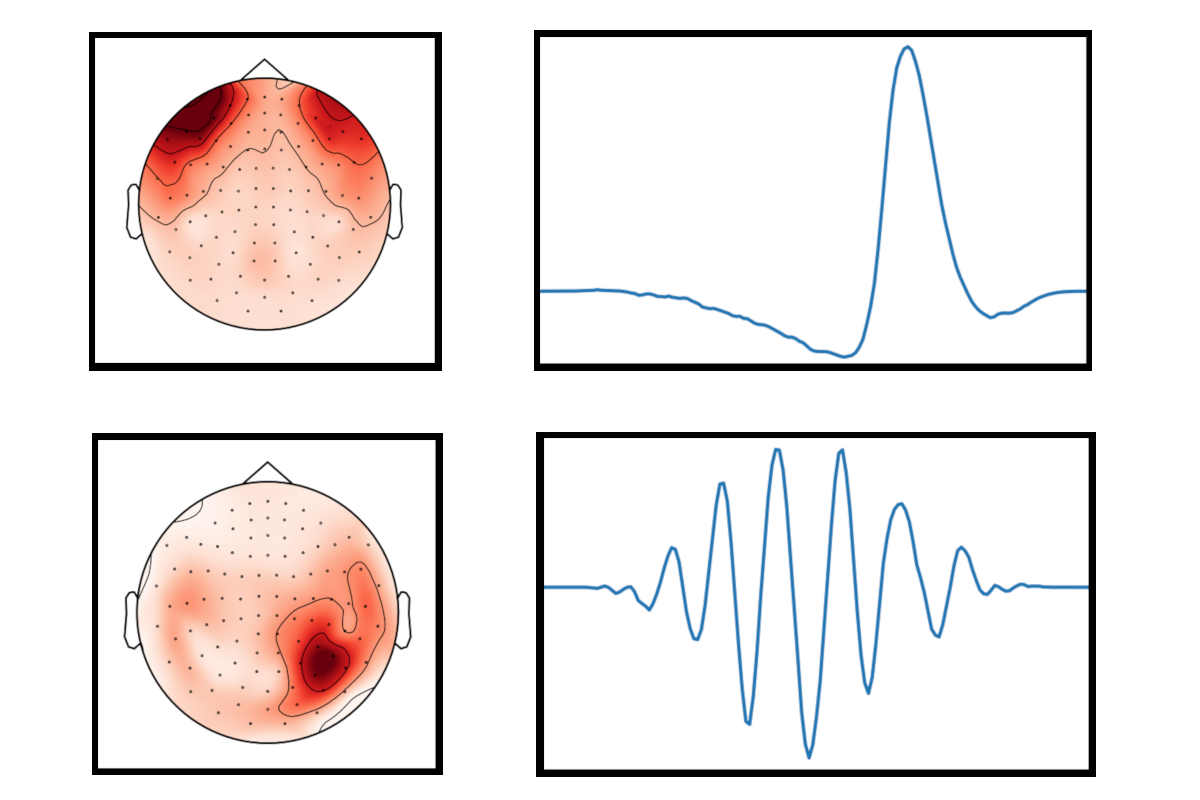
\includegraphics[width=6em]{meg_dict}
    };}
    \draw[->, thick, shorten >= 3pt, shorten <= 3pt] (signal.east) -- (dict.west)
            node[midway, align=center] {
                \footnotesize Dictionnaire\\
                \alt<-1>{\footnotesize multivarié}{\footnotesize de rang 1}};
     \only<3>{
        \node[rounded corners=3pt, draw, above=0.4em of dict.center, fill=black!10] {\tiny Artefact};
        \node[rounded corners=3pt, draw, below=0.4em of dict.center, fill=black!10] {\tiny Réponse évoquée};
    }
\end{tikzpicture}\\[.5em]

{\setlength\bodywd{.9\linewidth} \highlight[c=linkcolor, wd=\bodywd]{
       Le signal est résumé mais les atomes ne sont pas compréhensibles}\\[1.5em]}

{\raggedright Pour une activité localisée, la propagation résultant des équations de Maxwell impose une {\bf structure de rang 1} pour le signal observé.\\[1em]}

$\Rightarrow$ Recherche d'atomes liés à des activités neuronales localisées\\[1em]
\highlight{Atomes avec un sens physique \color{black} \normalfont \eg{} réponses évoquées, artefacts}\\
\vspace{0pt plus 1 filll}{%

\includegraphics[height=.8em]{github}~\url{alphacsc.github.io}: librairie Python\\}
\end{frame}

\section{\textbf{Programme de recherche:}\\\color{black}\inserttitle}
\parttitleframe{}

\begin{frame}{Projet de recherche}


\begin{columns}[c]
\column{1em}
\rotatebox{90}{\Large Axe 1}
\column{.9\textwidth}
\begin{block}{\bf Modélisation pour les signaux en neurosciences}
    Identifier la structure dans le signal\\[.3em]
    \myitem{} Dépendance temporelle \hskip3ex \myitem{} Couplage fréquentiel\\[.3em]
\end{block}
\end{columns}
%
\vskip1em
\begin{columns}[c]
    \column{1em}
    \rotatebox{90}{\Large Axe 2}
    \column{.9\textwidth}
    \begin{block}{\bf Analyse statistique des modèles convolutifs non supervisés}
        Évaluer les modèles non supervisés\\[.3em]
        \myitem Garantie de reconstruction \hskip2ex\myitem Algorithme global\\[.3em]
    \end{block}
\end{columns}
%
\vskip1em
\begin{columns}[c]
    \column{1em}
    \rotatebox{90}{\Large Axe 3}
    \column{.9\textwidth}
    \begin{block}{\bf Apprentissage profond pour les problèmes inverses}
        Lien entre modèle convolutif et apprentissage profond\\[.3em]
        \myitem Résolution rapide \myitem{} Identifiabilité de l'apprentissage profond\\[.5em]
    \end{block}
\end{columns}

\end{frame}

\setbeamercovered{transparent}

\begin{frame}[t]{Modélisation pour les signaux en neurosciences \keypoint{Axe 1}}
\begin{columns}[T]
    \column{.5\textwidth}
    \centering
    \textbf{Comment mettre à jour les dépendances temporelles?}

    \vskip1em
    \centering
    \setlength\bodywd{.9\linewidth}
    \highlight[wd=\bodywd]{Modéliser les interactions entre atomes}

    \alt<1-3>{
        \raggedright\vskip1.5em
         Pénalité $\ell_1$\\[.3em]
            \hskip2ex$\Rightarrow$ activations indépendantes\\[1em]
        \uncover<2->{Pénalités groupées (\eg{} $\ell_{1, 2}$)\\[.3em]
            \hskip2ex$\Rightarrow$ activations simultanées\\[1em]}
        \uncover<3->{Processus ponctuels (\eg{} Hawkes)\\[.3em]
            \hskip2ex$\Rightarrow$ interactions temporelles\\[1em]}
     }{
     \vskip.5em
     \highlight[wd=\bodywd]{Apprentissage auto-supervisé}\\

     \raggedright\vskip1.5em

     Prédiction de propriété \textit{ad hoc} \eg{}\\[.5em]

     \hskip1ex \raisebox{.1ex}{\small$\bullet$} à partir d'un segment, prédire T$_i$\\[.5em]
     \hskip1ex \raisebox{.1ex}{\small$\bullet$} prédire $\Delta t$ entre 2 segments\\[1em]

     \uncover<5>{{\bf Dictionnaire adapté à la tâche}\\[.3em]
                 \hskip1ex$\Rightarrow$ capture des effets temporels}
    }

    \column{.5\textwidth}
    \centering%
    \setlength\bodywd{.8\linewidth}
    \only<1>{

        \highlight[c=linkcolor, wd=\bodywd]{Activations indépendantes}\\[1em]
        \includegraphics[height=8em]{connectivity_independent.png}
        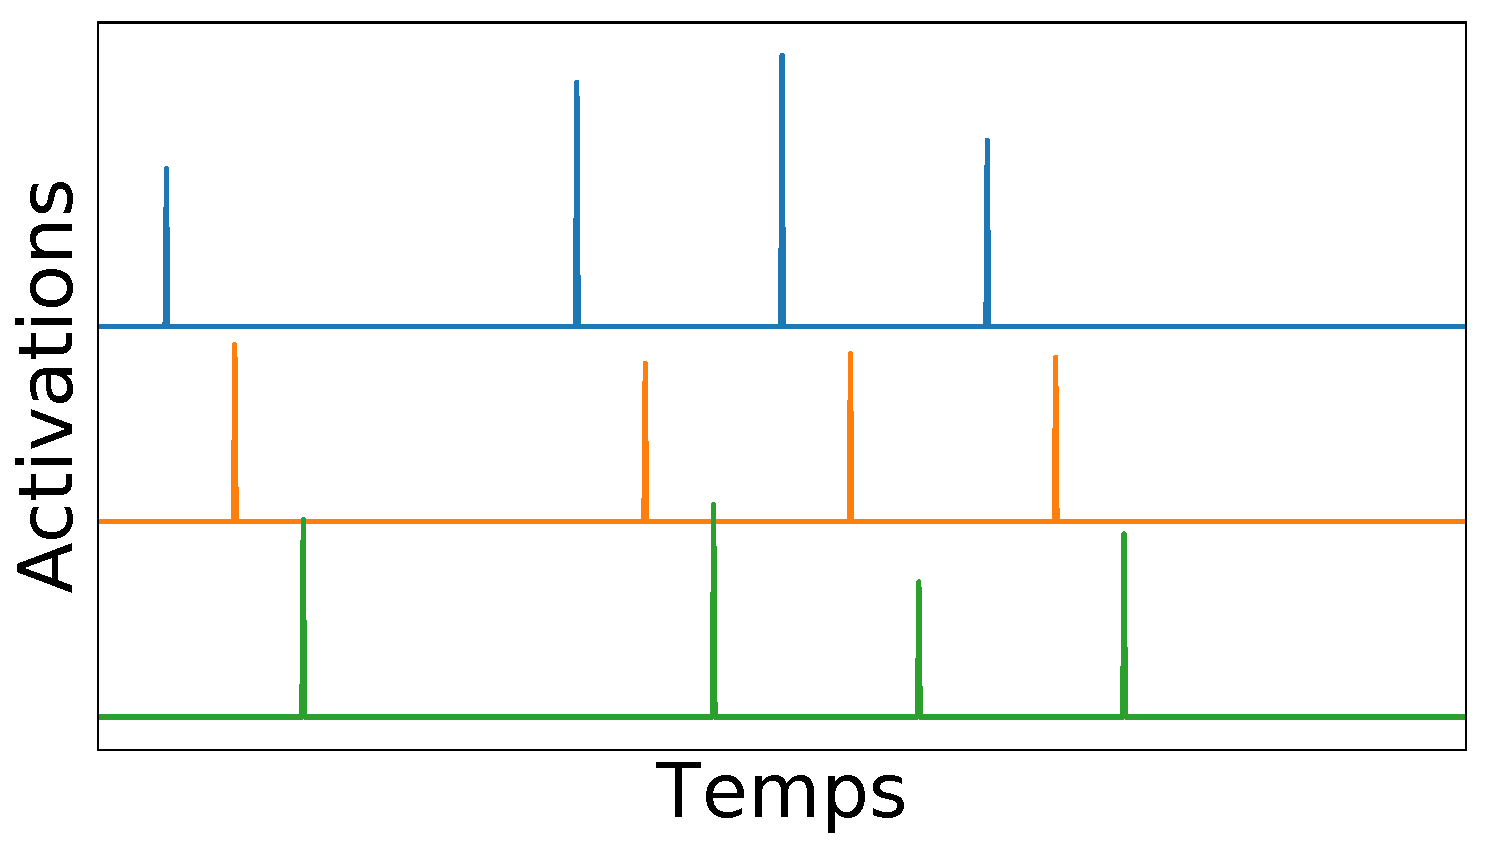
\includegraphics[width=\linewidth]{time_dependency}
    }%
    \only<2>{
        \highlight[c=linkcolor, wd=\bodywd]{Activations simultanées}\\[1em]
        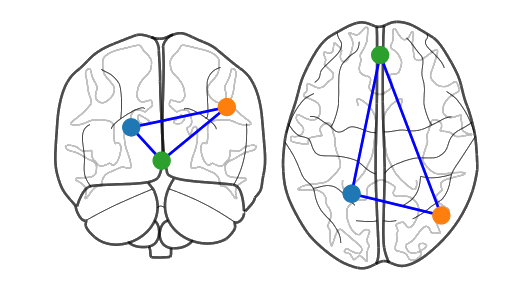
\includegraphics[height=8em]{connectivity_simultaneous.png}
        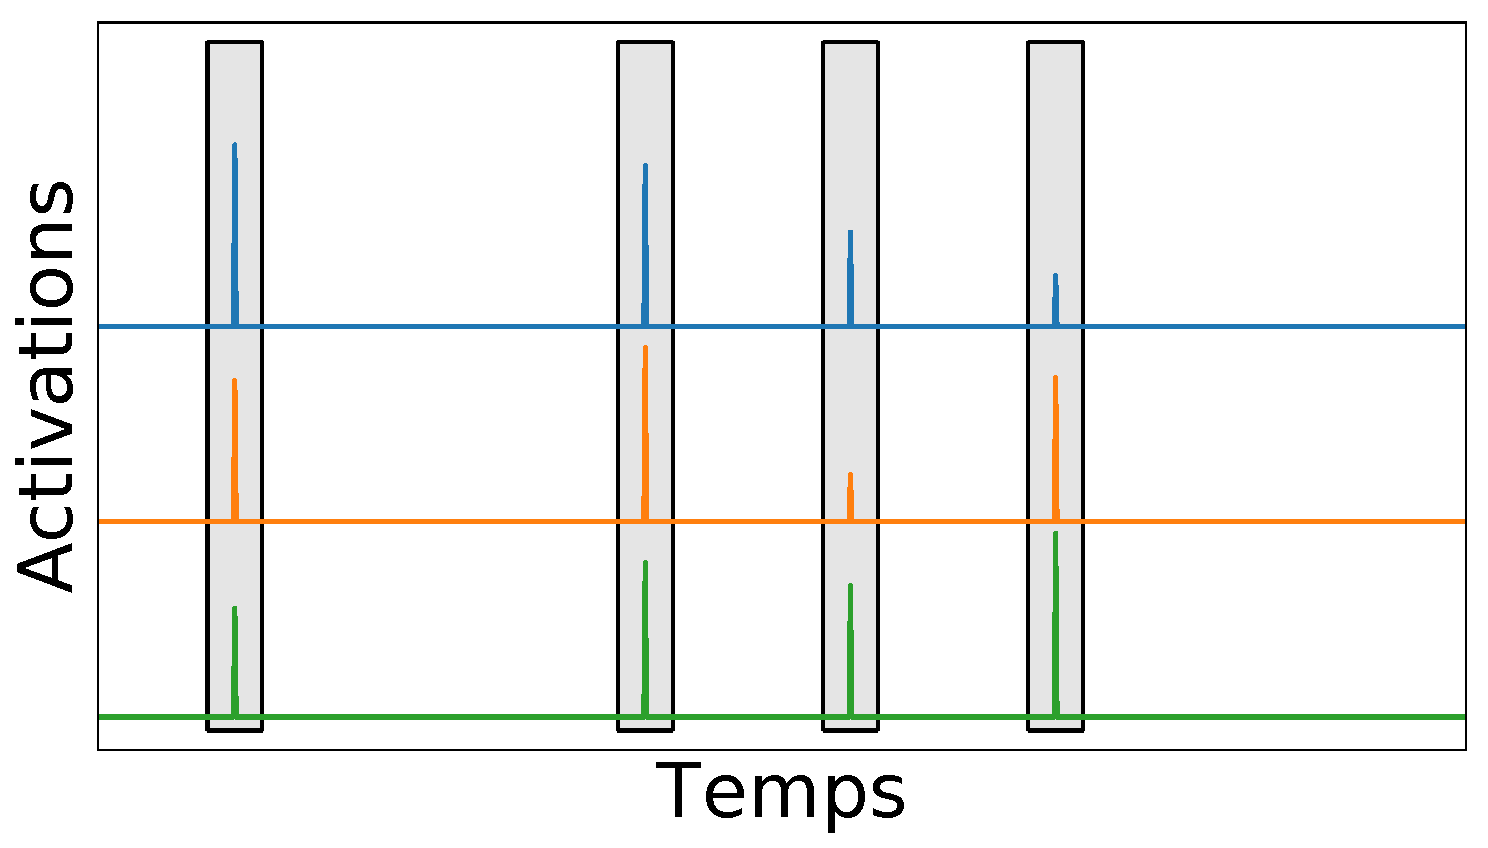
\includegraphics[width=\linewidth]{time_dependency_simultaneous}
    }%
    \only<3>{
        \highlight[c=linkcolor, wd=\bodywd]{Interaction temporelles}\\[1em]
        \includegraphics[height=8em]{connectivity_default_mode.png}
        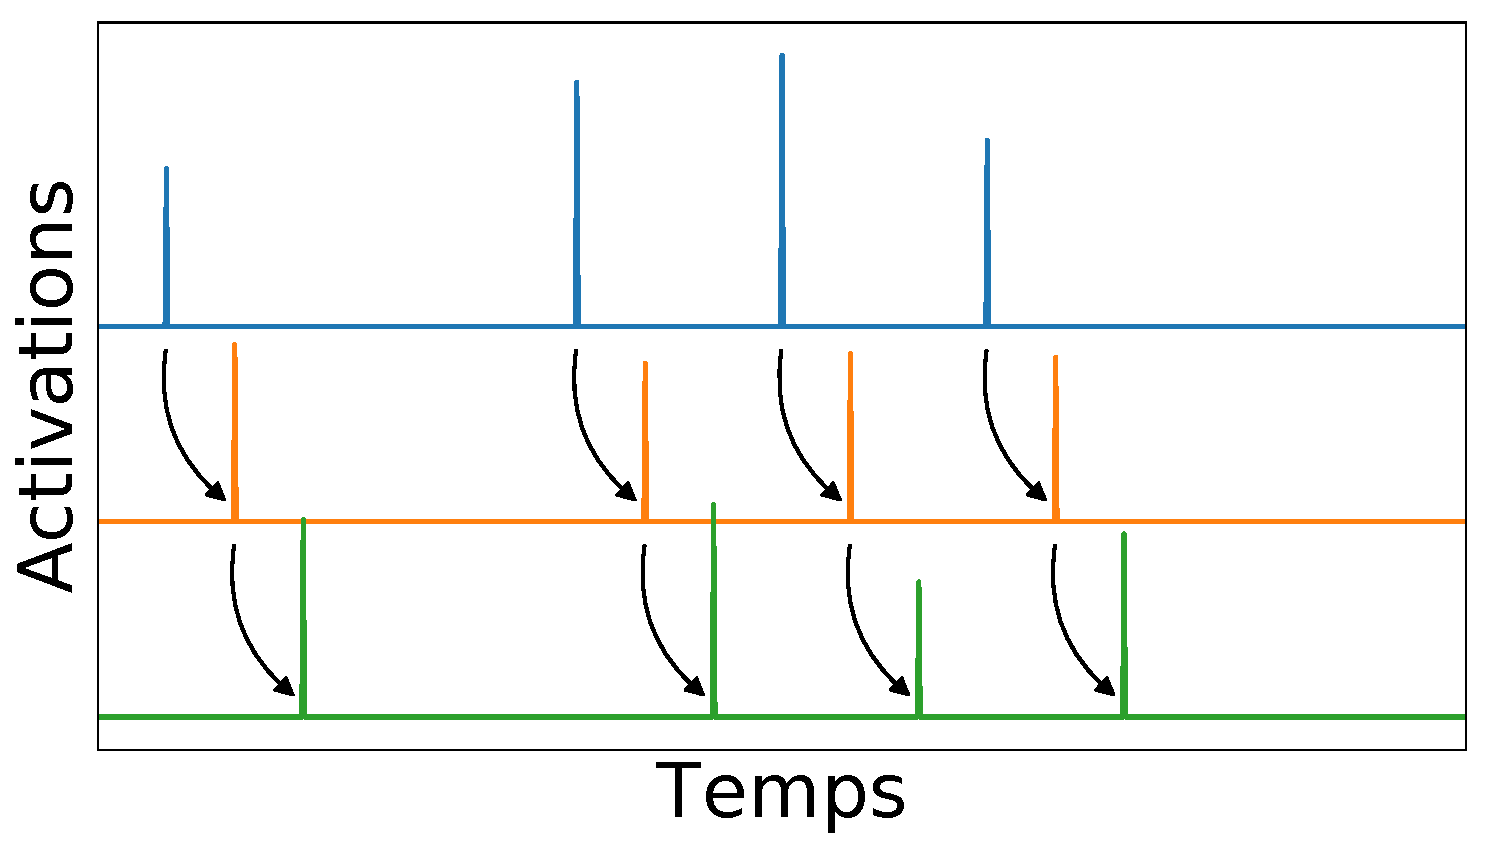
\includegraphics[width=\linewidth]{time_dependency_arrow}
    }%
    \only<4-6>{
        \highlight[c=linkcolor, wd=\bodywd]{Atomes non-stationnaires}\\[1em]
        \alt<5>{
            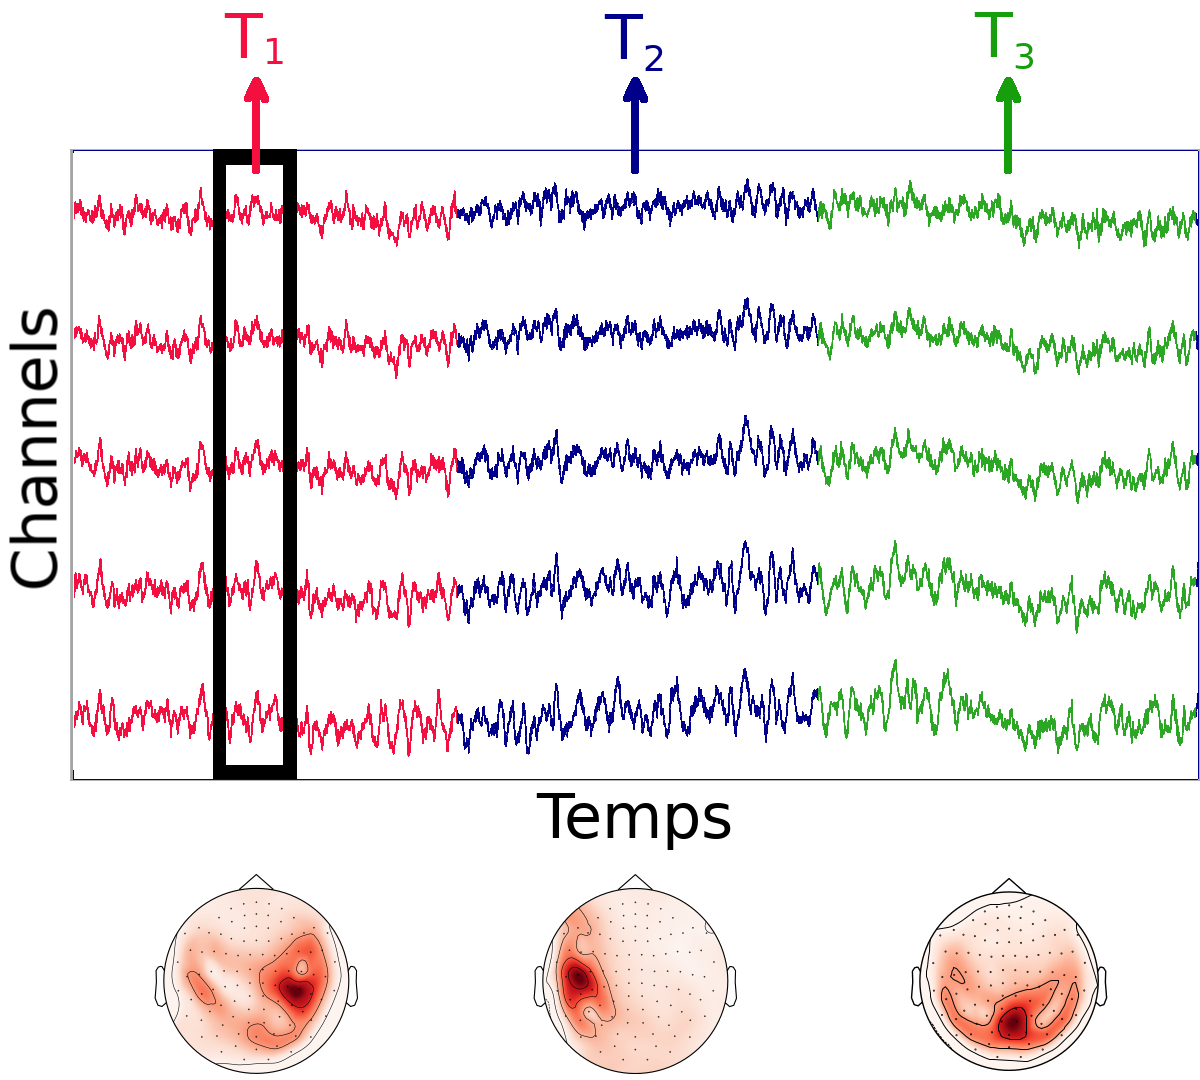
\includegraphics[width=\linewidth]{time_contrastive}
        }{
            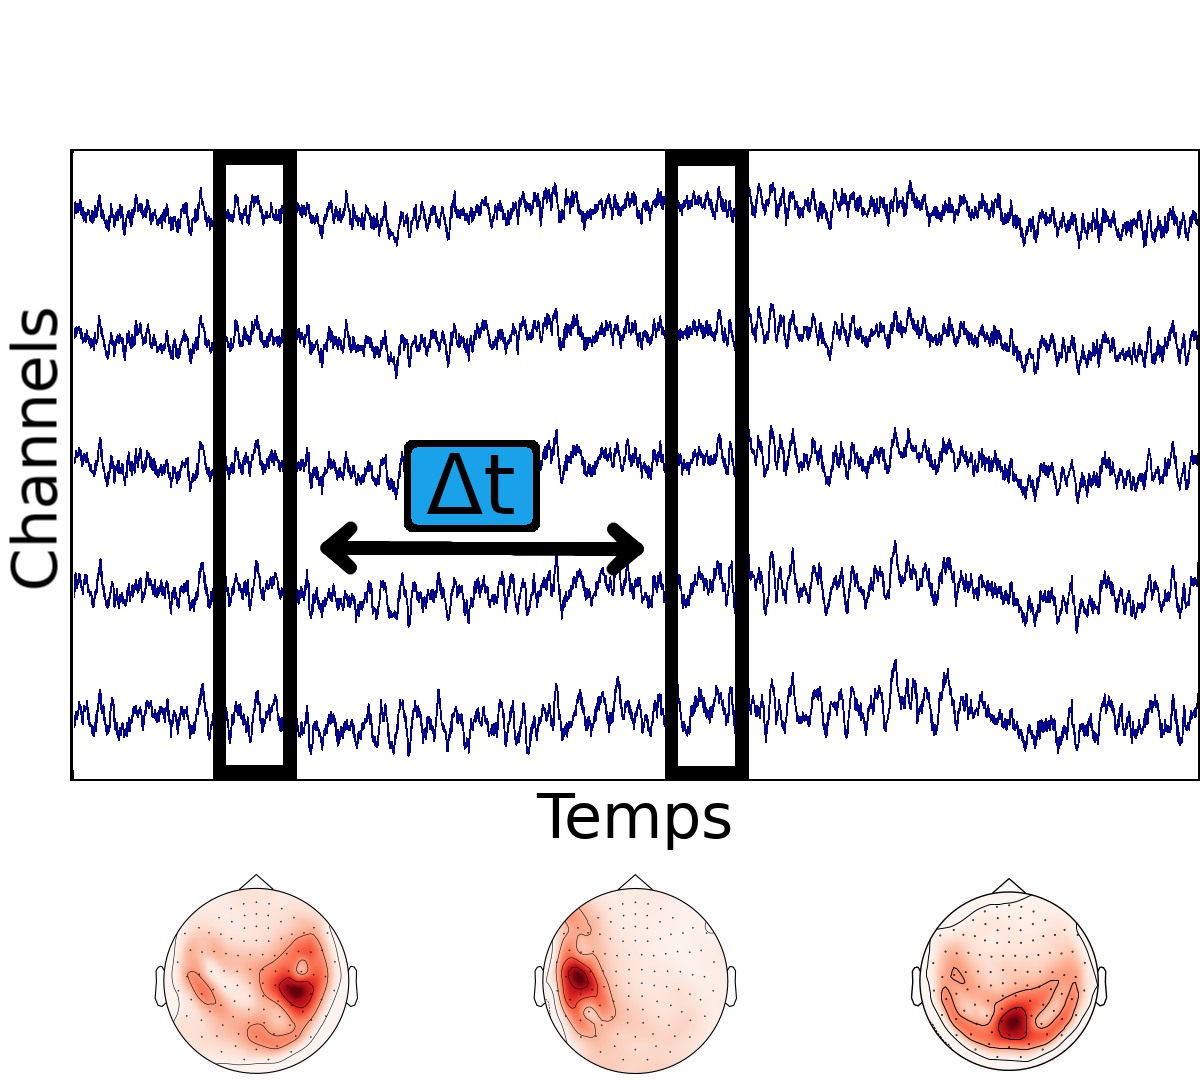
\includegraphics[width=\linewidth]{time_contrastive_delta_t}
        }\\[1em]
    }
\end{columns}

\end{frame}



\begin{frame}[t]{Analyse statistique des modèles non supervisés \keypoint{Axe 2}}

{\centering \textbf{Comment évaluer les modèles non supervisés?}\\[1em]}
\begin{tikzpicture}
    \coordinate (origin);
    \foreach \i in {0,...,2}{
        \node[inner sep=0em] (n\i) at (\i em, -\i em) {\includegraphics[width=4em]{meg_\i}};
    }

    \draw[densely dotted, <->, shorten >=1pt, shorten <=1pt] (n0.south west) -- (n2.south west);
         %node[midway, left] {N$_{\text{train}}$};

    \draw[->, black, thick, shorten >=3pt, shorten <=3pt] ($(n1.east) + (1em, 0)$) -- ++(5em, 0)
        node[midway, align=center] {\small Inférence\\[.2em]\textcolor{gray}{[{\color{linkcolor}Axe 1}]}}
        node[right] (atoms) {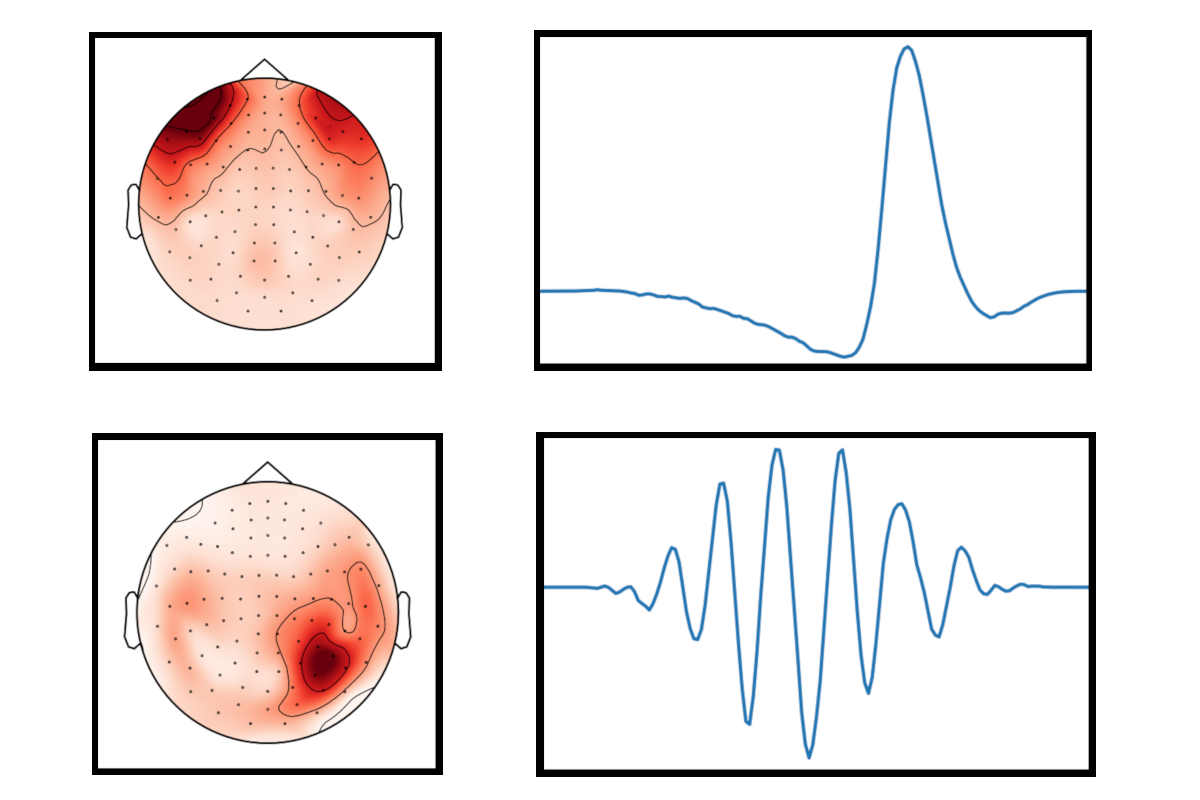
\includegraphics[width=5em]{meg_dict}};
    \draw[->, black, thick, shorten >=3pt, shorten <=3pt, dashed] (atoms.east) -- ++(6em, 0)
        node[midway, above] {\small Évaluation?}
        node[right, align=left, text width=5em] {Reconstruction?\\Débruitage?\\Génération?};

    % Labels
    \node[below=1em of n1, align=center] {\small Données\\\small d'entraînement};
    \node[below=0em of atoms] {\small Atomes};
\end{tikzpicture}
\vskip1em


\begin{columns}[c]

    \column{.3\textwidth}
    \centering

    \setlength\bodywd{\linewidth}
    \highlight[wd=\bodywd]{Garanties de reconstruction des atomes}\vskip1em
    \highlight[wd=\bodywd]{Convergence globale de l'inférence}

    \column{.65\textwidth}
    \setlength{\bodywd}{.95\linewidth}
    \centering
    \only<1>{%
        \highlight[c=linkcolor, wd=\bodywd]{Le modèle est-il identifiable?}\\[1em]
        {\hskip2ex\raggedright\bf Lien au spectre des atomes\\}
        \begin{itemize}
            \item Atome basse fréquence:\\bien reconstruit mais mal localisé
            \item Atome haute fréquence:\\mal reconstruit mais bien localisé
        \end{itemize}

    }%
    \only<2>{%
        \highlight[c=linkcolor, wd=\bodywd]{Le modèle peut-il être identifié?}\\[1em]
        {\hskip2ex\raggedright\bf Problème non convexe\\}
        \begin{itemize}
            \item Garanties d'optimalité globale\\pour la factorisation de matrice
            \item Approches gloutonnes pour la\\stabilisation de l'estimation
        \end{itemize}

    }%
\end{columns}
\end{frame}


\begin{frame}[t]{Apprentissage profond pour les problèmes inverses \keypoint{Axe 3}}

\centering
\definecolor{Z}{RGB}{45,162,65}
\definecolor{F}{RGB}{180,35,35}
\begin{tikzpicture}
    \node (meg) {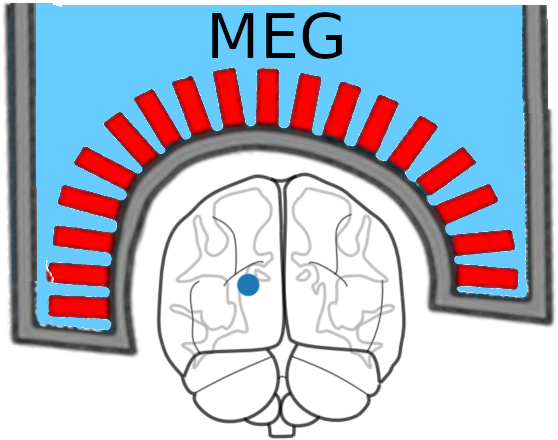
\includegraphics[width=9em]{meg_localised_source}};
    \draw[->, thick] ($(meg.east) - (0, 1.5em)$) -- ++(5em, 0)
        node[midway, align=center] (maxwell) {\small Équations\\ \small de Maxwell}
        node[right] (topomap) {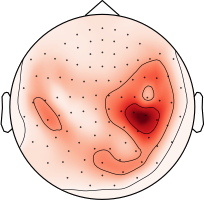
\includegraphics[width=4em]{topomap_somato}};
    \draw[->, thick] (topomap.east) -- ++(5em, 0)
        node[midway, align=center] {\small Problème\\ \small inverse}
        node[right] (brain) {\includegraphics[width=4em]{brain_activity}};
        \node[draw, rounded corners, above=2.5em] at (topomap.center) {
            \color{linkcolor} $\pmb X$};
        \node[draw, rounded corners, above=2.5em] at (brain.center) {
            \color{Z} $\pmb Z$};
        \node[draw, rounded corners, above=2.5em] at (maxwell.center) {
            \color{F} $\pmb F$};
\end{tikzpicture}

    {\bf Problème inverse:} $\argmin_{\color{Z} \pmb Z} \|{\color{linkcolor} \pmb X}
                         - {\color{F} \pmb F}{\color{Z} \pmb Z}\|_2^2
                         + \mathcal R({\color{Z} \pmb Z})$\\[1em]


\begin{columns}[T]
    \column{.4\textwidth}
    \centering{
        \setlength\bodywd{.9\linewidth}
        \highlight[wd=\bodywd]{\bf Résolution rapide de problème inverse}\\[.5em]
        \highlight[wd=\bodywd]{\bf Optimisation apprise}\\[.5em]
        \highlight[wd=\bodywd]{\bf Apprentissage profond identifiable}\\[.5em]
    }
    \column{.6\textwidth}

    \centering
    \only<1>{
        \begin{tikzpicture}
            \node (topomap) {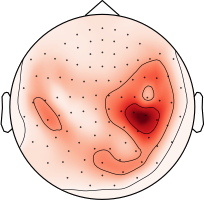
\includegraphics[width=4em]{topomap_somato}};
            \node[draw, rounded corners, above=2.5em] at (topomap.center) {
                \color{linkcolor} $\pmb X$};
            \draw[black, thick] ($(topomap.east) + (0, -3em)$) rectangle ++(1em, 6em)
                node[midway] (input) {};

            \draw[black, thick] ($(input.east) + (1.5em, -2.5em)$) rectangle  ++(1em, 5em)
                node[midway] (hidden) {};
            \draw[black, thick] ($(hidden.east) + (1.5em, -3.5em)$) rectangle ++(1em, 7em)
                node[midway] (output) {};

            \draw[dotted] ($(input.east) + (0, 3em)$) -- ($(hidden.west) + (0, 2.5em)$);
            \draw[dotted] ($(input.east) - (0, 3em)$) -- ($(hidden.west) - (0, 2.5em)$);

            \draw[dotted] ($(hidden.east) + (0, 2.5em)$) -- ($(output.west) + (0, 3.5em)$);
            \draw[dotted] ($(hidden.east) - (0, 2.5em)$) -- ($(output.west) - (0, 3.5em)$);

            \node[right=0.5em of output.east] (brain) {\includegraphics[width=4em]{brain_activity}};
            \node[draw, rounded corners, above=2.5em] at (brain.center) {
                \color{Z} $\pmb Z$};

            \node[rounded corners=3pt, fill=lightblue!70, draw=black, thick] at (hidden.center) {
                $f_\theta({\color{linkcolor} \pmb X})$};
        \end{tikzpicture}
        \setlength\bodywd{.95\linewidth}
        \highlight[c=linkcolor, wd=\bodywd]{%
            Les poids $\theta$ sont appris pour inverser $\color{F} \pmb F$}\\[1em]
    }
    \only<2>{%
        {\raggedright {\bf LISTA:} {optimisation apprise} \keypoint{ICLR 2017}\\[.5em]}
        \inputTikZ{.8}{ista_tikz}
        \vskip.3em
        \setlength\bodywd{\widthof{\bf Performances dépendent de la}}
            \highlight[c=linkcolor, wd=\bodywd]{Garantie pour la résolution des problèmes inverses?}\\[1em]
    }
%    \only<6>{
%
%        \setlength\bodywd{.9\linewidth}
%        \vskip3em
%        \highlight[c=linkcolor, wd=\bodywd]{Généralisation pour d'autres problèmes inverses\\[.3em]
%                                            \color{black}\normalfont$\Rightarrow$ Pénalité $\mathcal R$ différente de $\ell_1$}\\
%    }
    \only<3>{
        \begin{tikzpicture}
            \tikzset{
                boxe/.style={
                    rounded corners=3pt, ultra thick,
                    align=center, draw, text width=8em
                }
            }
            \coordinate (origin);
            \node[boxe, left=.5em of origin] (axe1) {\textbf{\color{linkcolor}Axes 1\&2}\\
                Modèles non supervisés {\bf identifiables}};
            \node[boxe, right=.5em of origin] (axe3) {\textbf{\color{linkcolor} Axe 3}\\
                Architecture pour les problèmes inverses};
            \node[boxe, text width=12em, below=4em of origin] (deep) {\textbf{Auto-encodeurs\\profonds identifiables}};
            \draw[->, thick, shorten >=3pt] (axe1.south) -- ($(deep.north) - (2em, 0)$);
            \draw[->, thick, shorten >=3pt] (axe3.south) -- ($(deep.north) + (2em, 0)$);
        \end{tikzpicture}
    }

\end{columns}

\end{frame}


%===========================================================================
\section{Conclusion}
%===========================================================================


\begin{frame}{Intégration dans l’équipe/collaborations}

\begin{columns}[c]
%    \column{1em}
%    \rotatebox{90}{}
    \column{\linewidth}
    \begin{beamercolorbox}[rounded=true, shadow=true]{title}
        \vskip-.1em%
        {\color{black} \bf Parietal}\\[.3em]
        Modélisation neurophysiologique: \textcolor{linkcolor}{A. Gramfort; P. Ciuciu; D. Engemann}\\[.3em]
        Évaluation non supervisée: \textcolor{linkcolor}{B. Thirion; G. Varoquaux}\\[.3em]
        Problèmes inverses rapides : \textcolor{linkcolor}{P. Ciuciu; A. Gramfort}\\[.3em]
    \end{beamercolorbox}
\end{columns}


\vskip.5em
\begin{columns}[c]
%\column{1em}
\column{\linewidth}
\begin{beamercolorbox}[rounded=true, shadow=true]{title}
    \vskip-.1em%
    {\color{black}\bf Nationales}\\[.3em]
    Charactérisation des nystagmus chez le nourrisson:\\
        \hskip1em\textcolor{linkcolor}{M. Robert (CHU Necker); L. Oudre (UP13); P.-P. Vidal (Descartes)}
\end{beamercolorbox}
\end{columns}


\vskip.5em
\begin{columns}[c]
%\column{1em}
\column{\linewidth}
\begin{beamercolorbox}[rounded=true, shadow=true]{title}
    \vskip-.1em%
    {\color{black} \bf Internationales}\\[.3em]
    Modélisation neurophysiologique: \textcolor{linkcolor}{B. Olshausen (Berkeley)}\\[.3em]
    Lien apprentissage profond et problème inverse: \textcolor{linkcolor}{J. Bruna (NYU)}\\[.3em]
\end{beamercolorbox}
\end{columns}


\end{frame}


\begin{frame}[t]{Apprentissage non supervisé pour les données de santé}%
\setlength{\parskip}{0em}
%
\begin{columns}[c]
    \column{2em}
    %\rotatebox{90}{\bf \large Parcours}%
    \column{.9\textwidth}%
    \begin{beamercolorbox}[rounded=true, shadow=true]{title}%
    {\large \bf \color{black} Parcours}\\
    2010-2014: X \hskip5.5em 2013-2014: Telecom ParisTech - MVA\\
    2014-2017: ENS Cachan \hskip.9em 2018-2019: Inria -- Parietal
\end{beamercolorbox}
\end{columns}%
%
\vskip.7em
\begin{columns}[c]
    \column{2em}
    \rotatebox{90}{\parbox{4em}{\centering\large \bf Maths\\appli}}
    \column{.9\textwidth}%
    \begin{beamercolorbox}[rounded=true, shadow=true]{title}
\begin{columns}[c]
    \column{.85\textwidth}
        Méthodes non supervisées et structure locale des signaux\\
        Lien apprentissage profond et optimisation\\
        \keypoint{3 publications dans les conférences les plus sélectives}
    \column{.15\textwidth}
        \includegraphics[height=3em]{brain_and_signals}
\end{columns}
\end{beamercolorbox}
\end{columns}
\vskip.7em
\begin{columns}[c]
    \column{2em}
    \rotatebox{90}{\parbox{4em}{\centering\bf \large Données\\Santé}}
    \column{.9\textwidth}%
    \begin{beamercolorbox}[rounded=true, shadow=true]{title}
    \begin{columns}[c]
        \column{.62\textwidth}
            Analyse de la marche \keypoint{2 articles; 1 brevet}\\
            Mouvements oculaires \keypoint{3 articles soumis}\\
            Neurosciences \keypoint{2 actes de conférence}\\
        \column{.38\textwidth}
            \centering
            \includegraphics[height=3em]{logo_cognac}
            \includegraphics[height=3em]{logo_neurospin}
    \end{columns}
    \end{beamercolorbox}
\end{columns}
\vskip.7em
\begin{columns}[c]
    \column{2em}
    \rotatebox{90}{\parbox{4em}{\centering\bf \large Logiciel\\Libre}}
    \column{.9\textwidth}%
    \begin{beamercolorbox}[rounded=true, shadow=true]{title}
        \begin{columns}[c]
            \column{.03\textwidth}
            \column{.47\textwidth}
            Calcul parallèle en Python\\
            Développeur pour 3 librairies\\
            Contributeur pour 2 projets
            \column{.5\textwidth}
            \centering
            \includegraphics[height=3em]{logo_python}
            \includegraphics[height=3em]{logo_joblib}
            \includegraphics[height=3em]{logo_sklearn}
        \end{columns}
    \end{beamercolorbox}
\end{columns}

\end{frame}

%===========================================================================
% AUXILIARY SLIDES
%===========================================================================



%===========================================================================
\appendix
\section{Auxiliary Slides}
%===========================================================================


%===========================================================================
\subsection{Aux1}
%===========================================================================
%
%\begin{frame}{LISTA}
%
%\end{frame}
%\begin{frame}{BOLD IRMf}
%
%\end{frame}
%\begin{frame}{LISTA}
%
%\end{frame}
%
%
%\begin{frame}{}
%\vskip2em
%{\centering
%    \usebeamercolor[fg]{title}
%    \usebeamerfont{title}
%    \Huge \bf Merci!\\[2em]}
%
%Code available online:\\[1em]
%
%%
\includegraphics[height=.8em]{github}~\textbf{LISTA} : github.com/tommoral/AdaptiveOptim\\[1em]
%
%
\includegraphics[height=.8em]{github}~\textbf{alphacsc} :  \url{alphacsc.github.io}\\[2em]
%
%Slides are on my web page:\\[1em]
%\hskip5em\includegraphics[height=.8em]{website} \url{tommoral.github.io}
%\hskip4em 
\includegraphics[height=.8em]{twitter} \href{https://twitter.com/tomamoral}{@tomamoral}
%
%
%\end{frame}
%

\end{document}
